%%%%%%%%%%%%%%%%%%%%%%%%%%  ltexpprt.tex  %%%%%%%%%%%%%%%%%%%%%%%%%%%%%%%%
%
% This is ltexpprt.tex, an example file for use with the SIAM LaTeX2E
% Preprint Series macros. It is designed to provide double-column output.
% Please take the time to read the following comments, as they document
% how to use these macros. This file can be composed and printed out for
% use as sample output.

% Any comments or questions regarding these macros should be directed to:
%
%                 Donna Witzleben
%                 SIAM
%                 3600 University City Science Center
%                 Philadelphia, PA 19104-2688
%                 USA
%                 Telephone: (215) 382-9800
%                 Fax: (215) 386-7999
%                 e-mail: witzleben@siam.org


% This file is to be used as an example for style only. It should not be read
% for content.

%%%%%%%%%%%%%%% PLEASE NOTE THE FOLLOWING STYLE RESTRICTIONS %%%%%%%%%%%%%%%

%%  1. There are no new tags.  Existing LaTeX tags have been formatted to match
%%     the Preprint series style.
%%
%%  2. You must use \cite in the text to mark your reference citations and
%%     \bibitem in the listing of references at the end of your chapter. See
%%     the examples in the following file. If you are using BibTeX, please
%%     supply the bst file with the manuscript file.
%%
%%  3. This macro is set up for two levels of headings (\section and
%%     \subsection). The macro will automatically number the headings for you.
%%
%%  5. No running heads are to be used for this volume.
%%
%%  6. Theorems, Lemmas, Definitions, etc. are to be double numbered,
%%     indicating the section and the occurence of that element
%%     within that section. (For example, the first theorem in the second
%%     section would be numbered 2.1. The macro will
%%     automatically do the numbering for you.
%%
%%  7. Figures, equations, and tables must be single-numbered.
%%     Use existing LaTeX tags for these elements.
%%     Numbering will be done automatically.
%%
%%  8. Page numbering is no longer included in this macro.
%%     Pagination will be set by the program committee.
%%
%%
%%%%%%%%%%%%%%%%%%%%%%%%%%%%%%%%%%%%%%%%%%%%%%%%%%%%%%%%%%%%%%%%%%%%%%%%%%%%%%%



\documentclass[twoside,leqno,twocolumn]{article}
\usepackage{ltexpprt}
\usepackage{parskip}
\usepackage[inline]{enumitem}
\usepackage{amsmath}

\newcommand{\Tau}{\mathrm{T}}

\begin{document}


%\setcounter{chapter}{2} % If you are doing your chapter as chapter one,
%\setcounter{section}{3} % comment these two lines out.

\title{\Large Classifying Vehicles From Automatic Number \\ Plate Recognition Camera Scans}
\author{Pedro M. Pinto Silva \thanks{School of Computing Science, Newcastle University, United Kingdom}
\and
Matthew Forshaw\footnotemark[1]
\and
Stephen McGough\footnotemark[1]}
\date{}

\maketitle

% Copyright Statement
% When submitting your final paper to a SIAM proceedings, it is requested that you include
% the appropriate copyright in the footer of the paper.  The copyright added should be
% consistent with the copyright selected on the copyright form submitted with the paper.
% Please note that "20XX" should be changed to the year of the meeting.

% Default Copyright Statement
\fancyfoot[R]{\footnotesize{\textbf{Copyright \textcopyright\ 2018 by BigTraffic\\
Unauthorized reproduction of this article is prohibited}}}

% Depending on which copyright you agree to when you sign the copyright form, the copyright
% can be changed to one of the following after commenting out the default copyright statement
% above.

%\fancyfoot[R]{\footnotesize{\textbf{Copyright \textcopyright\ 20XX\\
%Copyright for this paper is retained by authors}}}

%\fancyfoot[R]{\footnotesize{\textbf{Copyright \textcopyright\ 20XX\\
%Copyright retained by principal author's organization}}}


%\pagenumbering{arabic}
%\setcounter{page}{1}%Leave this line commented out.

\begin{abstract} \small\baselineskip=9pt This is the text of my abstract. It is a brief
description of my
paper, outlining the purposes and goals I am trying to address.\end{abstract}


% !TEX root = paper.tex
\section{Introduction}

The volume of traffic on our roads has been growing steadily for over 25 years, both in terms of the number of vehicles on the road -- increasing by 40.6\% in the UK~\cite{noVehiocles} -- and the distances covered -- 325.5 billion miles driven in the UK in the year ending September 2017 which is up nearly 30\% in the last 25 years~\cite{distance}. This is placing ever more burden on the road infrastructure along with those who police and manage it. In order to better understand how we can deal with this increase in demand we need to better understand how the road network is being used. By understanding road usage we can better deal with congestion, handle traffic incidents, plan road modifications and deal with illegal acts.

In a utopian model we would have full disclosure of all journeys made by all vehicles on the road infrastructure. However, this has numerous ethical and technical issues. From an ethical standpoint should we be allowed to know where all vehicles are at any given point in time. From a technical point of view, although every vehicle could be fitted with a GPS tracker -- costly in its own right -- there would still exist the issue of how we would collect and stream all of this data for future processing. Alternatively one can view the problem the other way around and rather than tracking individual vehicles look at collecting information by observing vehicles passing points within the road networks. A prime example of this approach are Automatic Number Plate Recognition (ANPR) cameras. These cameras are a combination of digital camera coupled with Artificial Intelligence to identify number plates within the image and convert these into strings of characters. ANPR cameras are normally fixed in location\footnote{Although cameras can be in a vehicle and moved from location to location.} able to view all vehicles passing that location.

For ANPR the problem now becomes that of recovering as much information about vehicle's journey as possible from the limited number of observations. ANPR cameras are normally located on major roads and interchanges, however, this only covers a tiny fraction of the road network. We can, though, estimate routes between cameras by understanding the distances between cameras and the most ``sensible'' routes between them. This allows us, given a set of ANPR sightings of the same vehicle, to produce a ``most likely'' route for that journey. It should be noted that we cannot determine the actual start and end of the journey as these will happen in areas not covered by ANPR. It should also be noted that for ethical reasons it is not normal to obtain actual number plates, but rather the hash of these. Though, for most situations this will suffice.

Once we have a set of sightings of a vehicle using ANPR, we now need to convert these into actual journeys. The first requirement is to identify individual journeys. Although this can't be done with certainty we can apply general rules to distinguish one journey from the next. For example if two sightings are made from ANPR cameras which are connectable by a ``sensible'' route\footnote{Here ``sensible'' implies that a route between cameras A and B would not need to go through a third camera C.} in a time interval which is ``sensible'' then these can be determined to be part of the same journey. However, if the timings between two sightings is significantly longer than what would be expected then this would imply that the vehicle stopped between these two cameras and that the later sighting is part of a new journey. The process of journey identification needs to be performed on dirty data which contains numerous impurities which need to be handled. These include:

\begin{itemize}
	\item {\bf Number plate miss-reads:} Although ANPR cameras have accuracies of around 99, miss-reads are possible. This can lead to sightings being missed or vehicles being wrongly sighted in locations.
	\item {\bf Timing errors:} The time-stamps of sightings could be erroneous. The minor side of this is implausible journey times, though, more seriously, this can lead to reordering the set of cameras on a particular journey.
	\item {\bf Clones number plates:} For various reasons a number plate may be cloned and used on a different vehicle. This can lead to impossible journeys and journeys that the real vehicle did not make.
\end{itemize}

Once journeys have been identified from the sightings we can then progress by using these journeys to identify higher-order issues within the road network. In this paper we demonstrate how we can use this journey information in order to identify the most likely class each vehicle is a member of. By clustering over such characteristics as how many journeys are made each day, average length of journeys, the number of different ANPR cameras seen in a day and the times when journeys are made we can cluster vehicles into buses, taxis, commuters and delivery vehicles.

The rest of this paper is presented as follows. In Section \ref{s.related} we discuss related work. Section \ref{s.ncl} we presents the ANPR data for the Newcastle area. Our process for identifying individual journeys is presented in Section \ref{s.trips} while Section \ref{s.classification} presents our classification approach. We present results in Section \ref{s.results} before offering conclusions and future directions in Section \ref{s.conclusions}.

\section{Related Work}
\label{s.related}

\begin{figure}[t]
\centering
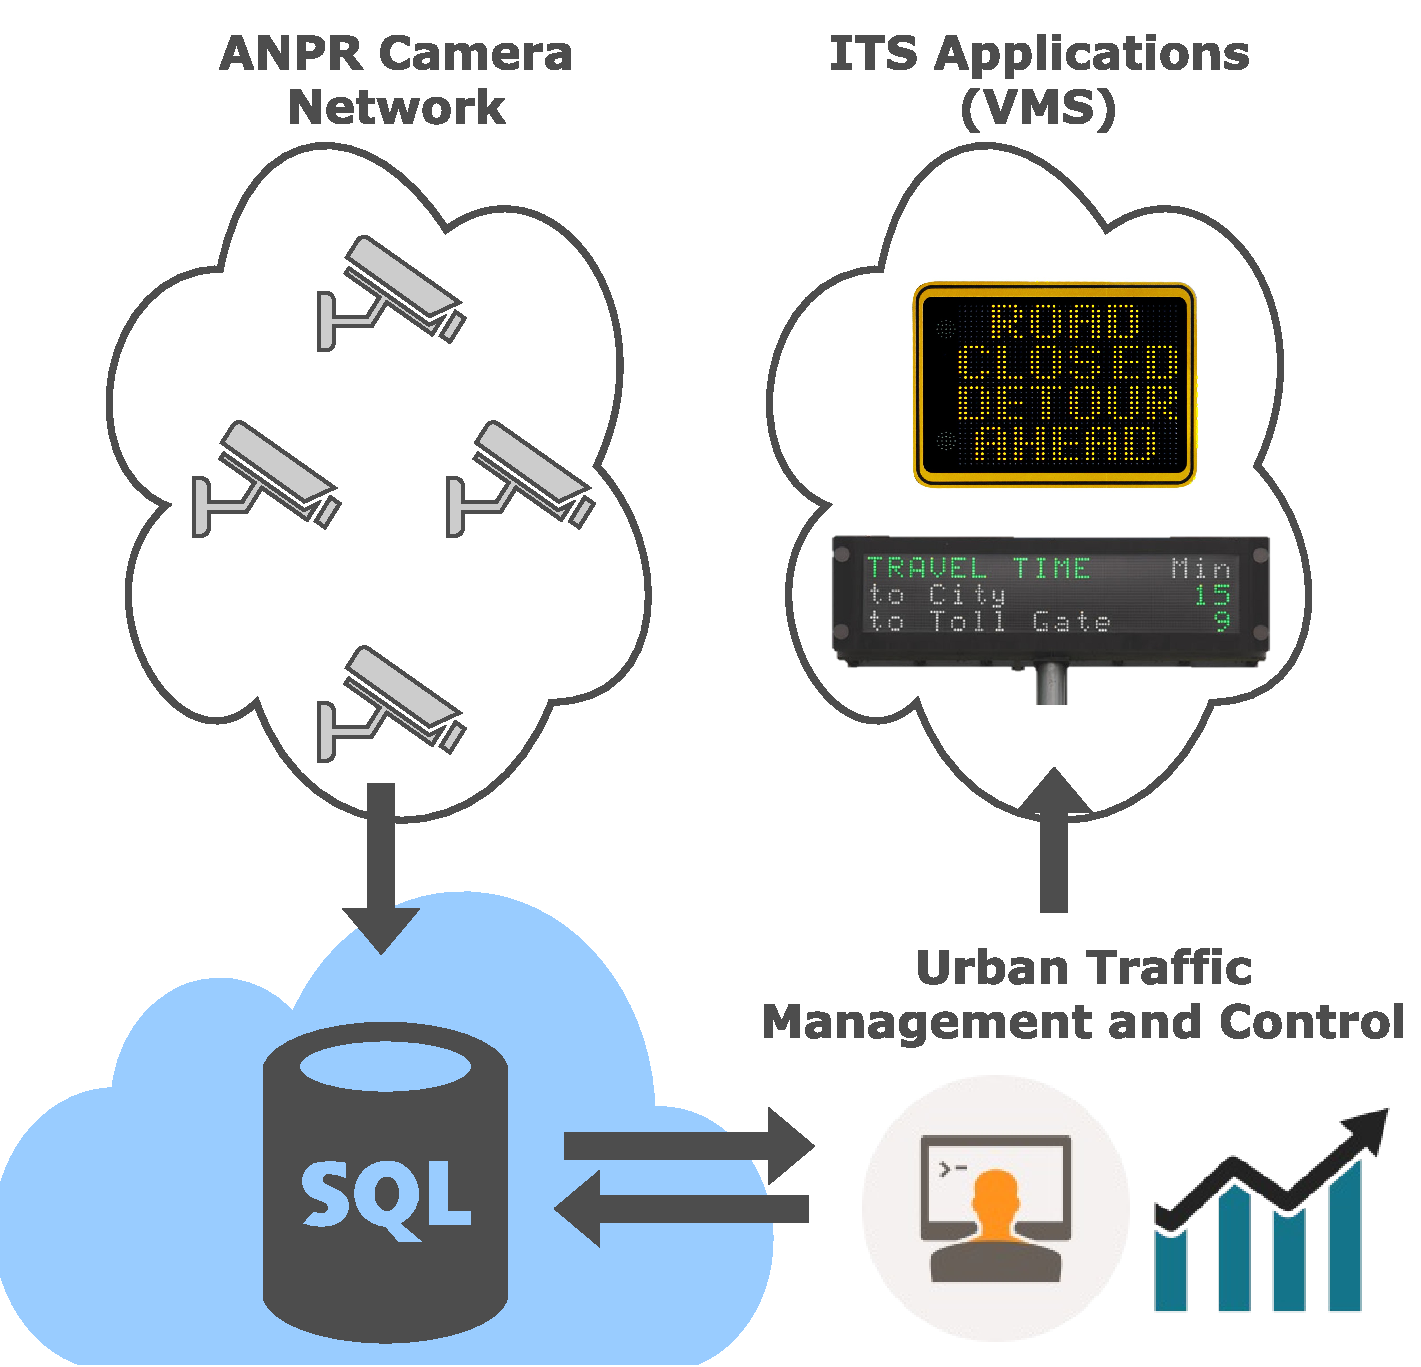
\includegraphics[width=.90\linewidth]{ANPR-overview.pdf}
\caption{Overview of a ANPR-based system for traffic monitoring and control.}
\label{fig:anpr-overview}
\vspace{-0.6cm}
\end{figure}

The main use of ANPR data for the UTMC is estimating average journey times for selected or sensitive links in the road network. Furthermore, several authors have extensively researched how to use number plate data as an extension to link counts for estimating origin-destination matrices and link flows~\cite{Castillo2010, Castillo2008, Hazelton2012}. However, very few works have focused on analysing individual or collective travel patterns from number plate data, particularly across extended periods of time. Moreover, there is no consistent conceptual and analytical framework for transforming number plate data into a historical sequence of trips for each vehicle. Finally, we believe that trip data, properly identified from number plate data, has the potential to unlock a number of new applications for urban traffic control and law enforcement. Thus, in section~\ref{s.trips} we present a conceptual methodology for grouping multiple camera observations of the same vehicle into one or several trips of that vehicle.

Determining the distribution of travel modes is one of the fundamental steps in the four-stage model: an essential traffic modelling methodology for transportation planning~\cite{FourStepModel}. Previous works have used trip information derived from different sources of data to identify travel mode or purpose of trip. More notably, survey data, floating car data and mobile phone data have been used~\cite{ODMobileData, ClusteringGPS}.  Although number plate data has been used in~\cite{Clustering} to identify different categories of trips, the authors do not differentiate between private or public travel modes and focus instead on categorising trips by time of occurrence. Hence, in section~\ref{s.classification} we apply the \emph{k-means} clustering algorithm to derived trip data and based on the results, we discuss the limitations of proposed methods and that of ANPR data.

% However, Furthermore, ANPR cameras can either be fixed or

% {\color{red}Uses of trip data for understanding travel demands / traffic prediction
%
% Studies about best placement of cameras
%
% Number plate data is not as popular, for urban traffic monitoring and prediction, as other sources of data, namely GPS traces or floating vehicle data.
% Previous works trips from GPS traces, .
%
% %Therefore, number plate scans provide additional trip information, besides simple link counts, that has
%
%  %estimating travel demands and traffic states. extended traditional methods of  travel demands
%
%
% Although significant research has gone into identifying trips from GPS traces, to the best of our knowledge, little research has gone into doing so with number plate data. Therefore, the contributions of this paper are twofold:

% \begin{enumerate}
%   \item
% \end{itemize}


% !TEX root = paper.tex
\section{Trip Identification}\label{s.trips}

Let the $i_{th}$ sighting of vehicle \emph{k} be defined as the unordered pair:

\begin{equation} \label{e.sighting}
s^{k}_{i} = \{ c, t \}
\end{equation}

where \emph{c} is an integer that uniquely identifies a camera, and \emph{t} is a scalar representing a point in time (e.g.\ a timestamp).

Let an ordered sequence of sightings of vehicle \emph{k} define the $u_{th}$ trip of \emph{k}:

\begin{equation} \label{e.trip}
w^{k}_{u} = \left(s^{k}_{(1)}, s^{k}_{(2)}, \dots , s^{k}_{(n)}\right)
\end{equation}

where \( n \) is the length of the trip, i.e.\ the number of sightings. Moreover, let the corresponding journey time sequence, of length \(n-1\), be defined as the time difference of consecutive sightings:

\begin{equation} \label{e.journeytime}
jt^{k}_{u} = \left(t^{k}_{(2)} - t^{k}_{(1)}, \ldots, t^{k}_{(n)} - t^{k}_{(n-1)} \right)
\end{equation}

We consider a trip of \emph{k} valid if the following conditions are met:

\begin{align}
n &\ge 1 , \label{e.trip.constraints.1} \\
\tau_{(i)} &< jt^{k}_{u(i)} < \Tau_{(i)} \ , \ \forall i \in jt^{k}_{u(i)} \label{e.trip.constraints.2}
\end{align}

The first condition~\ref{e.trip.constraints.1} is straightforward and specifies that every trip should have at least one sighting. The second condition~\ref{e.trip.constraints.2} defines a minimum and maximum travel times between consecutive observations. Its purpose is twofold:
\begin{enumerate*}[label=(\roman*)]
  \item first, to allow trips made by the same vehicle to be differentiated. For instance, given two consecutive sightings of \emph{k} three hours apart, we want to interpret them as belonging to different trips of \emph{k};
  \item second, it allows unplausible trips to be identified. For example, an unplausible trip can result from observing \emph{k} at a given camera and then a few seconds later at a second camera, several miles apart. Two explanations are common, either one of the cameras made a detection error, or there is another vehicle with a cloned plate number travelling in the road network.
\end{enumerate*} Evidently, condition~\ref{e.trip.constraints.2} is only valid for trips of length two or greater. Nevertheless, trips can easily be differentiated by first sorting sightings by time of occurrence, then calculating the journey time sequence for the entire sequence and finally comparing each element against $\Tau$. An example of a trip identified this way can be seen in Figure~\ref{fig:trip-example}.

\begin{figure}[t]
  \centering
  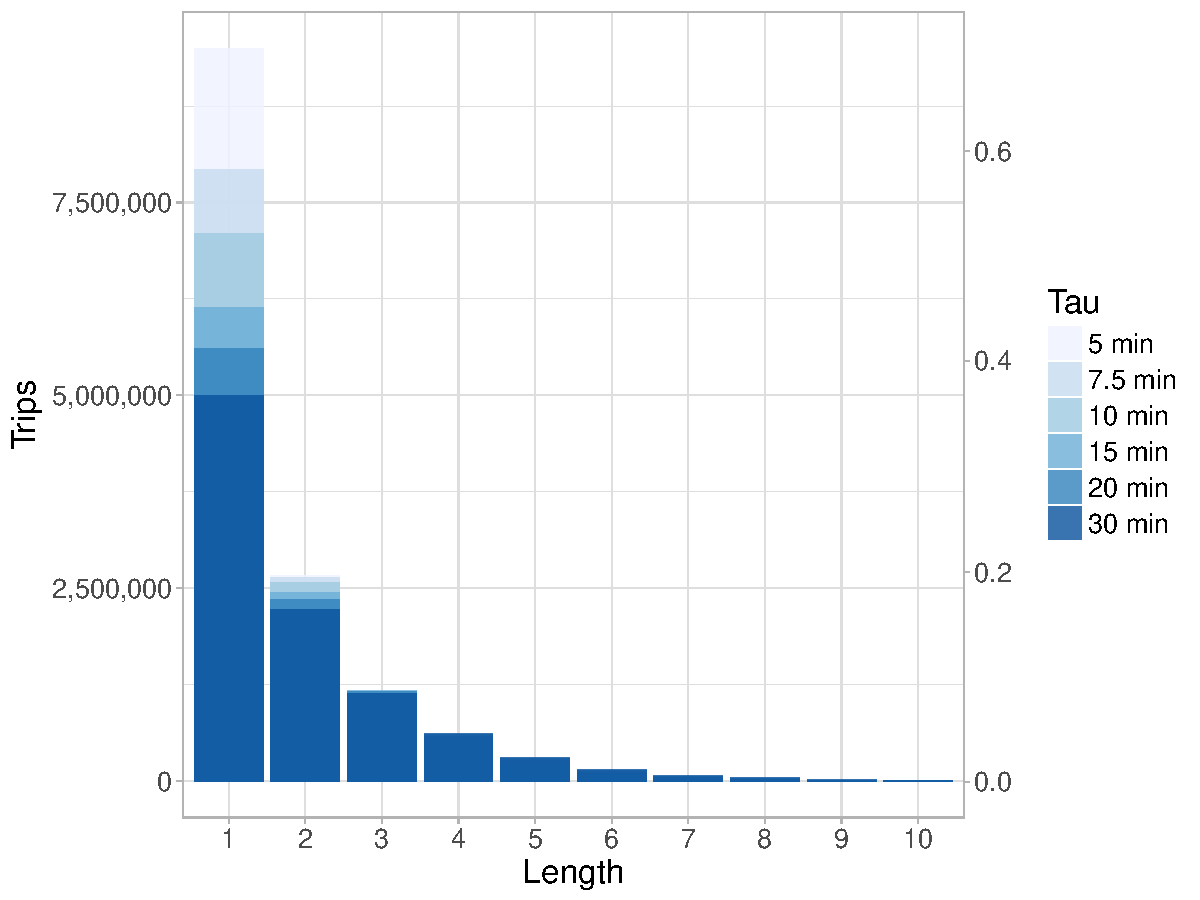
\includegraphics[width=1\linewidth]{length-dist.pdf}
  \caption{Distribution of trips per length of trip.}
  \label{fig:length-dist}
\end{figure}

\begin{figure*}[!ht]%
  \centering
  \begin{subfigure}[c]{.5\textwidth}
    \small
    \tabcolsep=0.09cm
    \begin{tabular}{c c c c c c c}
      \hline
      Vehicle & Camera & Timestamp & Trip & Sighting & \thead{Journey \\Time} & \thead{Trip \\Id}\\
      \hline
      2362920 & 1014 & \makecell{2017-02-01 \\ 00:00:06} &   1 &   1 & NA & 21 \\
      2362920 & 1044 & \makecell{2017-02-01 \\ 00:01:28} &   1 &   2 & 82.38 & 21 \\
      2362920 &  35 & \makecell{2017-02-01 \\ 00:02:32} &   1 &   3 & 63.50 & 21\\
      2362920 &  32 & \makecell{2017-02-01 \\ 00:04:38} &   1 &   4 & 125.95 & 21\\
       \hline
    \end{tabular}
    \label{fig:trip-example-table}
  \end{subfigure}\hfill
  %\qquad
  \begin{subfigure}[c]{.48\textwidth}
    \centering
    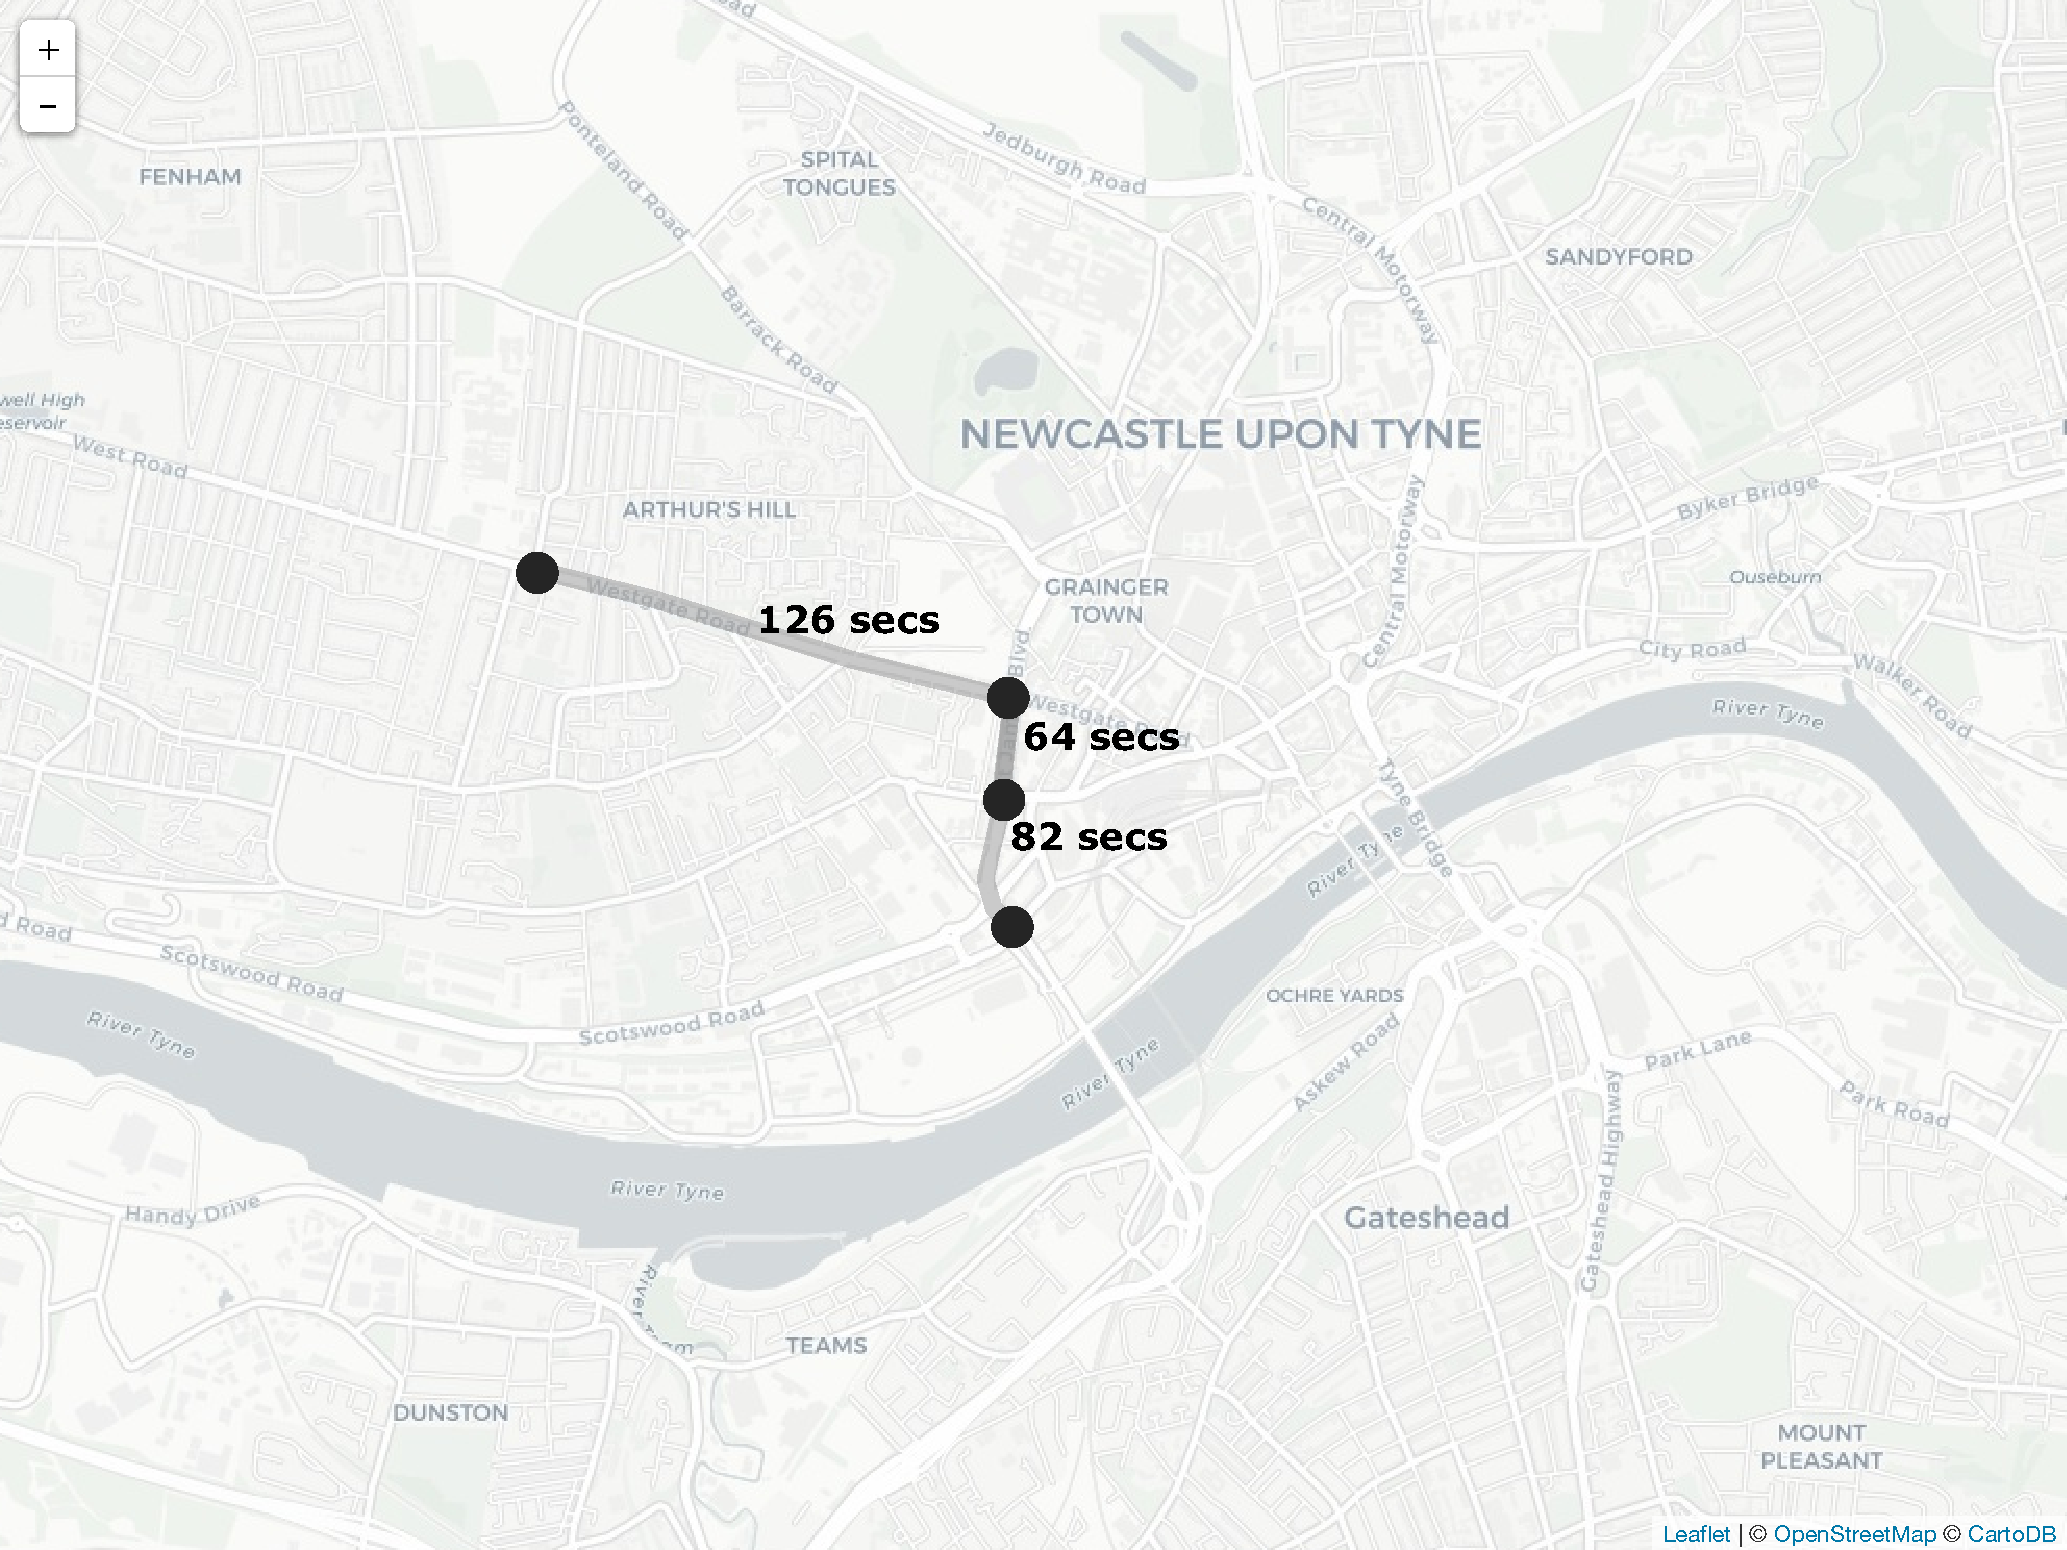
\includegraphics[width=1\linewidth]{trip-example.pdf}
    \label{fig:trip-example-map}
  \end{subfigure}\hfill
  \caption{Example of a trip of length 4. On the left side the correspoding data table is shown. The $u_{th}$ trip of each vehicle is given by the variable \emph{Trip}, whereas the $i_{th}$ sighting is given by variable \emph{Sighting}. The variable \emph{JourneyTime} gives the travel time from the previous to current sighting. Lastly, the variable \emph{TripId} represents the unique sequence of cameras that describes the trip. This allows trips to be grouped and summarised not only in terms of their origins and destination, but also routes. On the right side, the same trip is plotted on a map. However, the lines do not represent the true route taken by the vehicle, but instead the fastest driving route between sightings. Even though no routing information is available for each consecutive pair of sightings, the observed journey times can be compared against the distribution of collective journey times to rank the set of most likely routes chosen (which can be determined for instance by Stochastic User Equilibrium~\cite{Castillo2008}).}%
  \label{fig:trip-example}%
\end{figure*}

The simplest approaching to choosing the value of $\Tau$ is to pick a fixed empirical value, such as 5 or 10 minutes. However, if the distance between two cameras is greater than another origin-destination (od) pair of cameras, then it makes sense that $\Tau$ is relaxed. Similarly, if there is an anomaly in the road network, such as a traffic jam, and the routes connecting the two cameras are affected, then the value of $\Tau$ should also be adapted. Hence, $\Tau$ should be a function of the distance between the two cameras (or, more accurately, of the top n-routes between these) and the distribution of observed journey times. The same rationale can be applied to estimating $\tau$.

On the other hand, a consistent set of models and methodologies for estimating $\Tau$ and $\tau$, under a variety of circumstances and road anomalies, remains an open research problem. Thus, for the purposes of this work, we will consider these parameters to be fixed. Nevertheless, the importance of estimating these parameters should not be understated. Any errors in trip identification that occur due to poor estimation and filtering methods will propagate and be amplified in posterior analysis done using trip data. Therefore, $\Tau$ and $\tau$ estimation is something that needs to be carefully addressed and studied in the future in order to fully understand its impact in the outcome of the research. To briefly exemplify this, figure~\ref{fig:length-dist} shows how the number of trips per length of trip varies by fixing $\Tau$ at different empirical values ($\tau$ is ignored).

\subsection{Duplicate scannings}

To ensure that every trip of vehicle \emph{k} is unique in the sequence of all valid trips of vehicle \emph{k}:

\begin{align}
W^{k} = \left( w^{k}_{(1)}, w^{k}_{(2)}, \ldots, w^{k}_{(N)} \right) \label{e.trip.history}
\end{align}

where \emph{N} is the number of trips of \emph{k}, then there should be no two trips containing the same sighting:

\begin{align}
s^{k}_{(u(i))} \neq s^{k}_{(v(j))}, \forall u,v &= 1, 2, \ldots, N \ , \ u \neq v,  \label{e.trip.history.constraint} \\
\forall i,j &= 1, 2, \ldots, n \ , \ i \neq j \nonumber
\end{align}

However, ANPR can identify the same vehicle multiple times in the same run, if for instance the vehicle is stopped at a junction or traffic light. Hence, if two sightings occurred at the same location in a very short period of time, then there is a strong possibility that these are duplicate observations. As a simplification, we can assume that a trip should not contain cycles and that no camera should appear twice in the same trip. Yet, this assumption ignores cases where a vehicle is required to correct its route by passing through the same location as one previously observed in the same trip. Thus, we affirm that two sightings of vehicle \emph{k} are different if they were observed at two different points in time at different locations, or, if observed at the same location, then the time interval must be greater than a parameter $\gamma$, otherwise the two sightings are deemed as duplicates:

\begin{equation} \label{e.sighting.different}
t^{k}_{i} \ne t^{k}_{j} \Rightarrow s^{k}_{i} \ne s^{k}_{j} \ , \ i \ne j
\end{equation}

 Although the estimation of $\gamma$ carries similar considerations and consequences as those of estimating $\Tau$ and $\tau$, most duplicates can be identified in consecutive sightings of the same camera within the same trip. Even though a poor estimation of $\gamma$ also has impact in error propogation, this decreases substantially after filtering duplicates according to the heuristic above, due to the low occurrence of cycles in trips. Nevertheless, this issue needs to be fully investigated in future works.

\subsection{Errors in plate scanning}

Even though number plate recognition cameras have accuracy rates of 99.9\% or higher, on average 1 observation out of 1000 is a misclassified plate number. We categorise the errors made by ANPR cameras into two types:
\begin{enumerate}
  \item a passing vehicle is not detected by the camera;
  \item a different vehicle is detected instead.
\end{enumerate}
In the first case, there is no observed data. The corresponding trip sequence for the affected vehicle will be missing a sighting but we will have no indication of this. On the second case, there is a recorded sighting, but this will be assigned to the incorrect vehicle.


% !TEX root = paper.tex
\section{Clustering vehicles}\label{s.classification}

\begin{table*}[t]
\centering
\begin{tabular}{c c c c c c c c c c c}
  \hline
 \thead{Total\\Trips} & \thead{Average\\Trips} & \thead{Average\\Length} & \thead{Average\\Sightings} & \thead{Average\\Distinct\\Origins} & \thead{Average\\Distinct\\Destinations} & \thead{Average\\Distinct\\Routes} & \thead{Average\\First\\Hour} & \thead{Average\\Last\\Hour} & \thead{Average\\Hour\\Difference} & \thead{Average\\Rest\\Time} \\
  \hline
41 & 3.42 & 1.25 & 5.75 & 2.75 & 1.00 & 3.00 & 15.33 & 19.25 & 3.80 & 3.70 \\
3 & 1.50 & 1.00 & 1.50 & 1.50 & 0.00 & 1.50 & 14.00 & 14.50 & 0.73 & 0.73 \\
7 & 2.33 & 1.33 & 3.33 & 2.33 & 0.67 & 2.33 & 11.00 & 13.00 & 2.44 & 2.41 \\
12 & 2.40 & 1.10 & 3.60 & 2.40 & 0.60 & 2.40 & 14.40 & 16.40 & 2.00 & 1.95 \\
   \hline
\end{tabular}
\caption{Sample of extracted features from trips taken from 15 weekdays of number plate data.}
\label{t:features}
\end{table*}

One direct application of trip data is unsupervised learning. Previous works have focused on identifying travel modes or purpose of trip from different sources of data, most notably: survey data, GPS data and mobile phone data~\cite{ODMobileData, ClusteringGPS}. Determining the distribution of travel modes is one of the fundamental steps in the four-stage model: an essential traffic modelling methodology for transportation planning~\cite{FourStepModel}. Although number plate data has been used in~\cite{Clustering}, to identify different categories of trips, these do not differentiate between private or public travel modes and focus for the most part on when the trips occurred. Therefore, we aim to identify groups of vehicles with similar trip patterns based on frequency and diversity of travel. This can be private vehicles, such as work-home commuters, transit vehicles like buses and taxis, or other types of vehicles such as delivery trucks.
%This in turn, may enable trip modes to be estimated
However, due to its tiny coverage of the road network, it is not clear how well ANPR data can capture much the travel characteristics necessary to accurately describe the different groups.

Due to distinct traffic behavior during weekends, we chose to consider only trips occurring during weekdays. We thus used all number plate data collected during between the 6th and 24th of February and excluded data from the 2 weekends in between. Furthermore, as mentioned in section~\ref{s.trips}, we used fixed empirical values for $\Tau$, mostly due to time constraints. As such, we ran the trip identification sequence for the following values of $\Tau$: [5 , 7.5, 10, 15, 20, 30] minutes. The corresponding number of identified trips and average trip length is respectively [1.36M, 1.24M, 1.17M, 1.08M, 1.03M, 0.97M] and [1.46, 1.60, 1.69, 1.83, 1.92, 2.04]. Moreover, we did not set a value for $\tau$, but instead handled unplausible trips by filtering all sightings with confidence below 85\%. Duplicates were filtered after identifying consecutive sightings by the same camera occurring within the same trip. Clock synchronisation errors were provided in milliseconds with none exceeding 5 seconds. These were therefore ignored.

Transforming trips into features that could be used in clustering algorithms was a 3-step process:
\begin{enumerate}
  \item First, every trip was summarised as a single row of data. The following information was extracted: length of trip, origin, destination, route, start and end times.
  \item Second, daily trip information was obtained for each vehicle: number of trips, median of trip lengths, number of sightings, distinct number of origins destinations, and routes, hour of first sighting, hour of last sighting and total rest time between trips.
  \item Finaly, daily information per vehicle was collapsed into a single row by averaging this information across the 15 days.
\end{enumerate}

Table~\ref{t:features} depicts a sample of the resulting features vector. A total of 1034107 distinct vehicles were detected. However, because a high percentage of trips contains a single sighting, some of these features were highly correlated. We therefore, chose to remove 3 of the features represented in~\ref{t:features}: \emph{Average Sightings}, \emph{Average Distinct Routes} and \emph{Average Hour Difference}, to avoid the obfuscation of the natural clustering ~\cite{Kmeans}. Furthermore we considered that a trip of length 1 has no destination (which explains values of average distinct destination below zero) and we filtered all instances of vehicles where the total number of trips is lower than 3, resulting in 642006 unique vehicles.

Clustering of vehicles was performed using the Hartigan and Wong \emph{k-means} algorithm, for each value of $\Tau$. The number of clusters \emph{k} was varied between 2 and 8 and executed with 200 maximum iterations and 100 different starts of the algorithm. The Calinski-Harabasz criterion is used to pick the best value of $k$, the one that minimises the whithin-cluster and between-cluster errors and provides the more natural clusters ~\cite{Kmeans}. The results of vehicle clustering are presented and discussed in the section below.

\section{Results and Discussion}\label{s.results}

Table~\ref{t:tau_comparison} provides a summary of multiple runs of \emph{k-means} for each value of $\Tau$. The optimal number of clusters, selected by maximising the Calinski-Harabasz criterion, is presented and is shown to decrease inversely with $\Tau$. This in part expected because as $\Tau$ increases, so does the average trip length, as opposed to the total number of trips, and trips per vehicle.  The interp   ... The relative between and average whithin clusters sum of squares is also shown.

\begin{table}[ht]
\centering
\tabcolsep=0.17cm
\begin{tabular}{c c c c c}
  \hline
Tau & Best $k$ & Betweenss & \thead{Average\\Whithinss} & \thead{Calinski-\\Harabasz} \\
  \hline
5 min &   8 & 0.923 & 0.125 & 1,116,962 \\
  7.5 min &   7 & 0.904 & 0.143 & 1,003,744 \\
  10 min&   7 & 0.896 & 0.143 &   911,044 \\
  15 min &   6 & 0.865 & 0.167 &   794,557 \\
  20 min &   4 & 0.786 & 0.250 &   754,241 \\
  30 min &   3 & 0.710 & 0.333 &   743,001 \\
   \hline
\end{tabular}
\caption{\emph{k-means} performance for several values of $\Tau$.}
\label{t:tau_comparison}
\end{table}

Tables~\ref{t:kmeans_centers_450} and~\ref{t:kmeans_centers_1200} depict the cluster centers for $\Tau$ equal to 7.5 minutes and 20 minutes respectively. The values for the cluster centers partially meet our expectations. We were expecting to find a relatively small cluster representing taxis with a high average number of trips per day, occurring over a variety of origins and destinations and over a large time frame. Clusters 2 and 7 for $\Tau = 7.5$ and cluster 4 for $\Tau = 20$ do indeed fit this profile. What differentiates cluster 2 from 7 in the first case is essentially the mean number of trips per day and the average time at which the first and last trips of the day occur. We could expect that buses could be separated from taxis by showing less diversity in the number of origins and destinations as these essentially do multiple runs of the same trip throughout the day. Still, this can be explained by the fact that buses take routes through main and secundary roads. As most cameras are placed in main roads, the one long bus trip can be perceived as multiple small trips as the bus alternates between arterial and main roads.

On the other hand, we could expect that commuters display average and relatively few trips per day.

\begin{table*}[t]
\centering
\small
\begin{tabular}{c c c c c c c c c c}
  \hline
 Cluster &  Size & \thead{Total\\Trips} & \thead{Average\\Trips} & \thead{Average\\Length} & \thead{Average\\Distinct\\Origins} & \thead{Average\\Distinct\\Destinations} & \thead{Average\\First\\Hour} & \thead{Average\\Last\\Hour} & \thead{Average\\Rest\\Time} \\
  \hline
  1 & 108868 & 30.67 & 2.91 & 1.56 & 2.65 & 1.09 & 9.67 & 16.11 & 6.35 \\
  2 & 2948 & 170.08 & 13.69 & 1.47 & 9.20 & 4.67 & 6.89 & 18.69 & 11.65 \\
  3 & 309748 & 5.95 & 2.01 & 1.44 & 1.92 & 0.68 & 12.52 & 14.50 & 1.93 \\
  4 & 163982 & 16.99 & 2.30 & 1.46 & 2.13 & 0.77 & 11.12 & 14.99 & 3.81 \\
  5 & 45414 & 50.30 & 4.26 & 1.52 & 3.67 & 1.57 & 9.04 & 16.86 & 7.69 \\
  6 & 10380 & 86.99 & 7.16 & 1.43 & 5.55 & 2.49 & 8.41 & 17.60 & 9.03 \\
  7 & 666 & 331.50 & 26.43 & 1.57 & 9.31 & 5.17 & 5.73 & 19.59 & 13.14 \\
   \hline
\end{tabular}
\caption{Clusters sizes and mean centers for $\Tau = 7.5$ minutes.}
\label{t:kmeans_centers_450}
\end{table*}

\begin{table*}[t]
\centering
\small
\begin{tabular}{c c c c c c c c c c}
  \hline
 Cluster &  Size & \thead{Total\\Trips} & \thead{Average\\Trips} & \thead{Average\\Length} & \thead{Average\\Distinct\\Origins} & \thead{Average\\Distinct\\Destinations} & \thead{Average\\First\\Hour} & \thead{Average\\Last\\Hour} & \thead{Average\\Rest\\Time} \\
  \hline
  1 & 371318 & 7.19 & 1.76 & 1.68 & 1.68 & 0.71 & 12.30 & 14.55 & 2.14 \\
    2 & 49852 & 44.85 & 3.73 & 1.90 & 3.16 & 1.73 & 8.98 & 17.02 & 7.76 \\
    3 & 189224 & 22.82 & 2.29 & 1.84 & 2.11 & 1.06 & 10.00 & 15.76 & 5.60 \\
    4 & 4593 & 114.34 & 9.12 & 2.30 & 5.92 & 3.98 & 6.93 & 18.21 & 10.43 \\
   \hline
\end{tabular}
\caption{Clusters sizes and mean centers for $\Tau = 20$ minutes.}
\label{t:kmeans_centers_1200}
\end{table*}

The differences between expected and observed results are in great part due to the fact that a high percentage of trips contains a single sighting. .. It may be the case that commuters choose routes that do not pass through ANPR cameras. Devising further models and methods that model and capture this uncertainty is fundamental to getting the most out of ANPR data.


% !TEX root = paper.tex
\section{Conclusion and Future Work}\label{s.conclusions}

Most urban cities in the world possess a network of ANPR cameras that is used in law enforcement and for traffic monitoring and control. Number plate data collected in the Tyne and Wear area is stored and leveraged by the UTMC for computing average journey times across a selection of sensitive roads. However, number plate data could be used more extensively to identify and study individual and collective travel patterns. In this paper, we've presented a set of definitions and constraints that establish a conceptual foundation for identifying vehicle trips from number plate detections. We've identified two parameters, $\tau$ and $\Tau$ as critical in the discrimination of plausible and implausible trips. Hence, future work should first and foremost focus on developing formal methods to estimate these parameters from observed distributions of travel times and by applying knowledge about the structure of the road network. Moreover, methods for addressing issues concerning camera performance, namely wrong and duplicate scans, should be further developed and researched.

Once trip data has been computed, a range of interesting applications is available. This work tries to identify groups of vehicles by clustering information about frequency and diversity of travel. By associating a vehicle with a cluster that represents taxis, or home-to-work commuters, one can begin estimating trip mode usage across the city. However, the results presented here could benefit from extra work and further validation. Finally, future work can focus on using trip data to solve interesting research problems such as:
\begin{enumerate*}[label=(\roman*)]
  \item real-time route recommendation using probabilistic graphical models;
  \item detection of abnormal trip patterns for helping law enforcement in the identification of suspect vehicles or behavior;
  \item modelling how drivers make routing choices in the presence of anomalies in the road network.
\end{enumerate*}


\begin{thebibliography}{99}

\bibitem{SurveyITS2011}
Zhang, Junping, et al. {\em Data-driven intelligent transportation systems: A survey}. IEEE Transactions on Intelligent Transportation Systems 12.4 (2011): 1624-1639.

\bibitem{EvolutionUTMC2013}
Hamilton, Andrew, et al. {\em The evolution of urban traffic control: changing policy and technology}. Transportation planning and technology 36.1 (2013): 24-43.

\bibitem{Castillo2008}
Castillo, Enrique, José María Menéndez, and Pilar Jiménez. {\em Trip matrix and path flow reconstruction and estimation based on plate scanning and link observations}. Transportation Research Part B: Methodological 42.5 (2008): 455-481.

\bibitem{Hazelton2012}
Parry, Katharina, and Martin L. Hazelton. {\em Estimation of origin-–destination matrices from link counts and sporadic routing data}. Transportation Research Part B: Methodological 46.1 (2012): 175-188.

% \bibitem{BANKSMITH}
% R.~E. Bank and R.~K. Smith, {\em General sparse elimination requires no
%   permanent integer storage}, SIAM J. Sci. Stat. Comput., 8 (1987),
%   pp.~574--584.
%
% \bibitem{EISENSTAT}
% S.~C. Eisenstat, M.~C. Gursky, M.~Schultz, and A.~Sherman, {\em
%   Algorithms and data structures for sparse symmetric gaussian elimination},
%   SIAM J. Sci. Stat. Comput., 2 (1982), pp.~225--237.

\end{thebibliography}
\end{document}

% End of ltexpprt.tex
